\documentclass[aspectratio=169]{beamer}
\usetheme{focus}

%\usepackage{beamerthemesplit}
%\beamertemplatenavigationsymbolsempty
\usepackage{amsmath}
\usepackage{amsthm}
\usepackage{amssymb}
\usepackage{latexsym}
\usepackage{graphicx}
\usepackage{fancybox}
\usepackage{dsfont}
\usepackage{multirow} 
\usepackage{multicol}
\usepackage{booktabs} 
\usepackage{dcolumn}
\usepackage{soul}
\usepackage[cache=false]{minted}
\usepackage{MnSymbol}
\usepackage{stmaryrd}


\DeclareMathOperator*{\argmax}{arg\,max}
\DeclareMathOperator*{\argmin}{arg\,min}

\newcommand{\X}{\mathtt{X}}
\newcommand{\Y}{\mathtt{Y}}

%\newcommand{\R}{\mathbb{R}}
%\newcommand{\E}{\mathbb{E}}
%\newcommand{\V}{\mathbb{V}}
\newcommand{\p}{\mathbb{P}}
\newcommand*\df{\mathop{}\!\mathrm{d}}
\newcommand{\del}{\partial}


% imports
\usepackage{xargs}
\usepackage{xpatch}
\usepackage{etoolbox}
\usepackage{pdflscape}
\usepackage{booktabs}
\usepackage{threeparttable}
\usepackage[skip=0.2\baselineskip]{caption}

% command for inputting raw latex
\makeatletter
\newcommand\primitiveinput[1]{\@@input #1 }
\makeatother

% common table command
\newcommandx{\tablecontent}[4]{
    \begin{threeparttable}[!ht]
        \centering
        \caption{#3}
        \vspace{-1em}
        \footnotesize
        \begin{tabular}{#1}
            \primitiveinput{../tables/#2.tex}
        \end{tabular}
        \vspace{-0.2em}
        \begin{tablenotes}[flushleft]
            #4
        \end{tablenotes}
    \end{threeparttable}
}




% \usepackage{slashbox}
\title{Lecture 4: Bayesian Analysis}
\author{Chris Conlon }
\institute{NYU Stern }


\newcommand{\norm}[1]{\left\lVert#1\right\rVert}
\newcommand{\R}{\mathbb{R}}
\newcommand{\E}{\mathbb{E}}
\newcommand{\V}{\mathbb{V}}
\newcommand{\ol}{\overline}
%\newcommand{\ul}{\underline}
\newcommand{\pp}{{\prime \prime}}
\newcommand{\ppp}{{\prime \prime \prime}}
\newcommand{\policy}{\gamma}


\newcommand{\fp}{\frame[plain]}

\date{\today}

\begin{document}
\maketitle


\begin{frame}{Quick Refresh: Bayes Rule}
\begin{align*}
P(A | B)=\frac{P(B | A) P(A)}{P(B)}
\end{align*}
Given a \alert{positive test result} what is the probability a patient actually has cancer?
\begin{center}
\begin{table}[htp]
\caption{Test Accuracy}
\begin{center}
\begin{tabular}{l|r|r|}
& Cancer (1\%) & No Cancer (99\%) \\ \toprule
Positive Test& 80\% & 9.6\% \\
Negative Test& 20\% & 90.4\%
\end{tabular}
\end{center}
\end{table}%
\end{center}
\end{frame}


\begin{frame}{Quick Refresh: Bayes Rule}
Caclulate $Pr(Cancer \& Positive Test)$ and $Pr(No Cancer \& Positive Test)$
\begin{center}
\begin{table}[htp]
\caption{Joint Probabilities}
\begin{center}
\begin{tabular}{l|r|r|}
& Cancer (1\%) & No Cancer (99\%) \\ \toprule
Positive Test& (0.8)(0.01)=0.008 & (0.9)(0.096)=0.09504 \\
Negative Test& (0.2)(0.01)=0.002 & (0.9)(0.904)=0.89496
\end{tabular}
\end{center}
\end{table}
\end{center}
$Pr(Cancer | Positive Test) = \frac{Pr(Cancer, Pos Test)}{Pr(Cancer,Pos Test) + Pr(NoCancer, Pos Test)}= .008/.10304 = 0.0776$
\end{frame}



\begin{frame}{Introduction}
\begin{itemize}
\item Suppose that we toss a coin several times with $x_i \in \{H,T\}=\{1,0\}$ 
\item $\mathbf{X} = \{H,T,H,H,\ldots\}$.
\item Suppose that the probability of heads $Pr(x_i = H) = p$.
\item What is the likelihood of an observed sequence of $\mathbf{X}$? where $x_i$ are I.I.D.
\begin{align*}
Pr(x_i | p) &= p^{x_i} (1-p)^{1-x_i} \\
Pr(\mathbf{X} | p) &=  p^{\sum_i x_i} (1-p)^{\sum_i (1- x_i)} 
\end{align*}
\end{itemize}
\end{frame}

\begin{frame}{Introduction: MLE for coin toss}
Can construct the \alert{log likelihood} and find the MLE.
\begin{align*}
\ell(\mathbf{X} | p) &= (\sum_i  x_i ) \ln p + (N-\sum_i x_i) \ln (1-p)\\
\frac{\partial \ell(p) }{\partial p} &= (\sum_i  x_i ) \frac{1}{p} - (N-\sum_i x_i) \frac{1}{1-p} =0\\
\frac{1-p}{p}  &= \frac{(\frac{1}{N}\cdot N-\frac{1}{N}\cdot\sum_i x_i) }{\frac{1}{N}\cdot \sum_i x_i} \rightarrow \hat{p} = \frac{1}{N}\cdot \sum_i x_i
\end{align*}
\end{frame}


\begin{frame}{Introduction: MLE for coin toss}
Can also construct the properties of $\hat{p}$.
\begin{align*}
\mathbb{E}[\hat{p}] &= \mathbb{E} \left[ \frac{1}{N}\cdot \sum_i x_i \right]  = \left[ \frac{1}{N}\cdot \sum_i \mathbb{E} x_i \right]  = \mu_x = p_0\\
\mathbb{V}[\hat{p} | \mathbf{X}] &= \mathbb{V} \left[ \frac{1}{N}\cdot \sum_i x_i \right]  =  \frac{1}{N^2}\cdot \sum_i \mathbb{V} (x_i ) = \frac{N}{N^2} p (1-p)
\end{align*}
Which gives us a CI of:  $\left(\overline{x} \pm 1.96 \cdot \sqrt{\frac{1}{N} \overline{x} (1-\overline{x})} \right)$
\end{frame}

\begin{frame}{Bayesian Statistics: Brief Introduction}
A different idea:
\begin{itemize}
\item Start with a (diffuse) initial guess for the distribution of $p$: $f_P(p)$.
\item Incorporate information from likelihood: $f(x_i | p)$
\item Construct \alert{posterior density} estimate $f(p | x_i)$.
\begin{itemize}
\item This doesn't characterize a best estimate $\hat{p}$ but a full distribution.
\item We can calculate $\mathbb{E}[p | x_i]$ or $\mathbb{V}[p |x_i]$ or any other functions of the posterior density.
\end{itemize}
\item Challenge: How to choose initial $f_P(p)$.
\end{itemize}
\end{frame}



\begin{frame}{Bayesian Statistics: Brief Introduction}
One possible guess is the uniform distribution $f(x) = 0$ on $0 \leq x \leq 1$.
\begin{itemize}
\item \alert{Marginal/Prior Distribution}: $f_P(p) = 1$ for $0 \leq p \leq 1$.
\item \alert{Conditional Distribution}/Likelihood: $f_{X|P} (x | p) = p^x (1-p)^{1-p}$
\item \alert{Joint Distribution} : $f_{X,P}(x, p)=f_{X|P}(x | p)\cdot f_P(p)  = p^x (1-p)^{1-p}\cdot 1 = x \cdot p + (1-x) \cdot (1-p)$
\begin{itemize}
\item This is only defined for $p \in[0,1]$ and $x \in \{0,1\}$. It is zero elsewhere.
\end{itemize}
\item What about \alert{Marginal Distribution} for $x$?
\begin{align*}
\int _ { p } f _ { P X } ( x , p ) d p &= x \cdot \int _ { 0 } ^ { 1 } p d p + ( 1 - x ) \cdot \int _ { 0 } ^ { 1 } ( 1 - p ) d p \\
&= x \cdot \frac { 1 } { 2 } + ( 1 - x ) \cdot \frac { 1 } { 2 } = \frac { 1 } { 2 } \propto 1
\end{align*}
\end{itemize}
\end{frame}


\begin{frame}{Bayesian Statistics: Brief Introduction}
The object we are usually interested in is the \alert{Posterior Distribution}
\begin{align*}
f _ { P | X } ( p | x ) = \frac { f _ { X | P } ( x | p ) \cdot f _ { P } ( p ) } { \int _ { 0 } ^ { 1 } f _ { X | P } ( x | p ) \cdot f _ { P } ( p ) d p } = 2 p ^ { x } ( 1 - p ) ^ { 1 - x } \propto p ^ { x } ( 1 - p ) ^ { 1 - x }
\end{align*}
\begin{itemize}
\item We are back at the p.m.f. of the \alert{Bernoulli} which is maybe comforting.\\
\item This is true because $f_X(x) \propto 1$ and $f_P(p) \propto 1$.
\item $f _ { P | X } ( p | x=0) = (1-p)$ and $f _ { P | X } ( p | x =1)=p$.
\end{itemize}
\end{frame}

\begin{frame}{Bayesian Statistics: Beta-Prior}
\begin{itemize}
\item Let's try a different \alert{prior distribution} than the uniform we used last time. This time we will use a $Beta(\alpha,\beta)$ distribution:
\begin{align*}
f _ { P } ( p | \alpha,\beta) &= \frac { \Gamma ( \alpha + \beta ) } { \Gamma ( \alpha ) \cdot \Gamma ( \beta ) } p ^ { \alpha - 1 } ( 1 - p ) ^ { \beta - 1 }\\
\mathbb{E}[p | \alpha,\beta] &=\frac{\alpha}{\alpha + \beta}\\
\mathbb{V}[p | \alpha,\beta] &=\frac{\alpha \beta}{(\alpha + \beta)^2(\alpha+\beta+1)}
\end{align*}
\item This has the advantage that it places nicely with the Binomial.
\item Consider $\alpha=16, \beta=8$. This gives $\mathbb{E}[p ] = \frac{2}{3}$ and $\mathbb{SE}[p] = 0.094$. 
\end{itemize}
\end{frame}


\begin{frame}{Bayesian Statistics: Beta-Prior}
Consider the case where $x=1$ (we get one piece of new data).
\begin{align*}
f _ { P } ( p ) \cdot f _ { X | P } ( x | p ) =\underbrace{ \frac { \Gamma ( \alpha + \beta ) } { \Gamma ( \alpha ) \cdot \Gamma ( \beta ) }}_{C(\alpha,\beta)} p ^ { \alpha - 1 } ( 1 - p ) ^ { \beta - 1 } \cdot p \propto  p ^ { \alpha  } ( 1 - p ) ^ { \beta - 1 } 
\end{align*}
\begin{itemize}
\item The resulting distribution is now $(p|x=1)\sim Beta(\alpha+1,\beta)$.
\item Our posterior has mean $=0.68$ and SE $=0.091$.
\item Estimate of mean increases and SE decreases.
\item Likewise if $x=0$ we get $(p|x=0)\sim Beta(\alpha,\beta+1)$
\item There is a \alert{conjugacy} relationship between the Beta and the Binomial.
\end{itemize}
\end{frame}



\begin{frame}{General Case}
\begin{align*}
\overbrace{f_{\theta|X}(\theta | x)}^{\text{posterior}}=\frac{\overbrace{f_{X, \theta}(x, \theta)}^{\text{joint}}}{ \underbrace{f_{X}(x)}_{\text{marginal of } x}}
=\frac{\overbrace{f_{X|\theta}(x | \theta)}^{\text{likelihood}} \cdot  \overbrace{f_{\theta}(\theta)}^{\text{prior}}}{\int f_{X|\theta}(x | \theta) \cdot f_{\theta}(\theta) d \theta}
\end{align*}
There is a shortcut because the denominator doesn't depend on $\theta$
\begin{align*}
f_{\theta|X}(\theta | x) \propto f_{X|\theta}(x | \theta) \cdot f_{\theta}(\theta)=\mathcal{L}(\theta | x) \cdot f_{\theta}(\theta)
\end{align*}
We can cheat because there exists a constant $c$ so that $c \int \mathcal{L}(\theta | x) \cdot f_{\theta}(\theta) d \theta=1$.
\end{frame}

\begin{frame}{A Normal Example}
Assume $X \sim N(\mu,1)$ and $\mu \sim N(0,100)$. What is $f_{\mu | X}(\mu | X=x)$?
\begin{align*}
f_{\mu|X}(\mu | x) &\propto \exp \left(-\frac{1}{2}(x-\mu)^{2}\right) \cdot \exp \left(-\frac{1}{2 \cdot 100} \mu^{2}\right)\\
&=\exp -\frac{1}{2} (x^{2}-2 x \mu+\mu^{2}+\mu^{2} / 100) \\
&\propto \exp \left(-\frac{1}{2(100 / 101)}(\mu-(100 / 101) x)^{2}\right)
\end{align*}
It happens that $(u | x) \sim N(100x/101 , 100/101)$. \\
In general the posterior will not be well defined.
\end{frame}

\begin{frame}{Kalman Update: A More Complicated Normal}
Assume $X \sim N(\mu,\sigma^2)$ with $\sigma^2$ known. $\mu \sim N(\mu_0,\tau^2)$. What is $f_{\mu | X}(\mu | X=x)$?
\begin{align*}
f_{\mu|X}(\mu | x) &\propto \exp \left(-\frac{1}{2 \sigma^{2}}(x-\mu)^{2}\right) \cdot \exp \left(-\frac{1}{2 \cdot \tau^{2}}\left(\mu-\mu_{0}\right)^{2}\right)\\
&\propto \exp -\frac{1}{2}\left(\frac{x^{2}}{\sigma^{2}}-\frac{2 x \mu}{\sigma^{2}}+\frac{\mu^{2}}{\sigma^{2}}+\frac{\mu^{2}}{\tau^{2}}-\frac{2 \mu \mu_{0}}{\tau^{2}}+\frac{\mu_{0}^{2}}{\tau^{2}}\right)\\
&\propto \exp -\frac{1}{2}\left(\mu^{2} \frac{\sigma^{2}+\tau^{2}}{\tau^{2} \sigma^{2}}-\mu \frac{2 x \tau^{2}+2 \mu_{0} \sigma^{2}}{\tau^{2} \cdot \sigma^{2}}\right)\\
&\propto \exp -\frac{1}{2\left(1 /\left(1 / \tau^{2}+1 / \sigma^{2}\right)\right)}\left(\left(\mu-\left(x / \sigma^{2}+\mu_{0} / \tau^{2}\right) /\left(1 / \sigma^{2}+1 / \tau^{2}\right)\right)\right.
\end{align*}
The resulting distribution is Normal with mean and variance
\begin{align*}
\mathbb{E}[\mu | X=x]=\frac{\frac{x}{\sigma^{2}}+\frac{\mu_{0}}{\tau^{2}}}{\frac{1}{\sigma^{2}}+\frac{1}{\tau^{2}}}, \quad \frac{1}{\mathbb{V}(\mu | X)}=\frac{1}{\sigma^{2}}+\frac{1}{\tau^{2}}
\end{align*}
\end{frame}


\begin{frame}{Kalman Update: A More Complicated Normal}
Despite being a giant mess this makes sense:
\begin{align*}
\mathbb{E}[\mu | X=x]=\frac{\frac{x}{\sigma^{2}}+\frac{\mu_{0}}{\tau^{2}}}{\frac{1}{\sigma^{2}}+\frac{1}{\tau^{2}}}, \quad \frac{1}{\mathbb{V}(\mu | X)}=\frac{1}{\sigma^{2}}+\frac{1}{\tau^{2}}
\end{align*}
\begin{itemize}
\item Posterior mean is a weighted average of \alert{prior mean} and \alert{sample mean}.
\item Weights depend on \alert{precision} of two samples.
\item Posterior \alert{Precision} is sum of precision of each sample $\frac{1}{\mathbb{V}(\cdot)}$
\item Probably we want to choose a relatively \alert{uninformative} prior with large $\tau^2$.
\item $\tau^2 \rightarrow \infty$ implies an \alert{improper prior distribution} because it no longer integrates to one. But because of $\propto$ still mostly ok.
\end{itemize}
\end{frame}

\begin{frame}{Generalization to Multiple Observations}
This is straighforward:
\begin{align*}
p(\theta | X_{1}, \ldots, X_{N}) \propto \mathcal{L}(\theta | X_{1}, \ldots, X_{N}) \cdot p(\theta)
\end{align*}
\begin{itemize}
\item Still depends on: \alert{prior}, \alert{likelihood} to construct \alert{posterior}.
\item Can update one observation at a time or all at once.
\end{itemize}
\end{frame}

\begin{frame}{Frequentist Asymptotics for Bayesian Estimators}
\textbf{Bernstein von-Mises Theorem}
\begin{quote}
A posterior distribution converges as you get more and more data to a multivariate normal distribution centred at the maximum likelihood estimator with covariance matrix given by $n^{-1} I(\theta_0)^{-1}$, where $\theta_0$ is the true population parameter (Edit: here $I(\theta_0)$ is the Fisher information matrix at the true population parameter value).
\end{quote}
Under these conditions (and some more):
\begin{enumerate}
\item MLE is consistent
\item Fixed number of parameters
\item $\theta_0$ in interior of $\Theta$ (true value of SD can't $=0$).
\item The prior density must be non-zero in a neighborhood of $\theta_0$.
\item  log-likelihood needs to be smooth (two derivates at the true value and more)
\end{enumerate}
\end{frame}


\begin{frame}[fragile]{A (famous) Baseball Example}
Suppose we want to estimate batting averages $(AVG)$ for some baseball players
\begin{itemize}
\item $AVG = \frac{\# \text{hits}}{ \# At Bats}$
\item Use data on the first $n=45$ at bats and hits $x_i$ for the 1970 season.
\item Predict the batting average $\mu_i$ for the end of the season  ($n=400-500$ at bats).
\item Obvious estimate is batting average after 45 at bats: $\widehat{\mu}_i^{MLE}= x_i/45$.
\item Is there a better estimate?
\end{itemize}
\end{frame}


\begin{frame}[fragile]{A Baseball Example}
\begin{center}
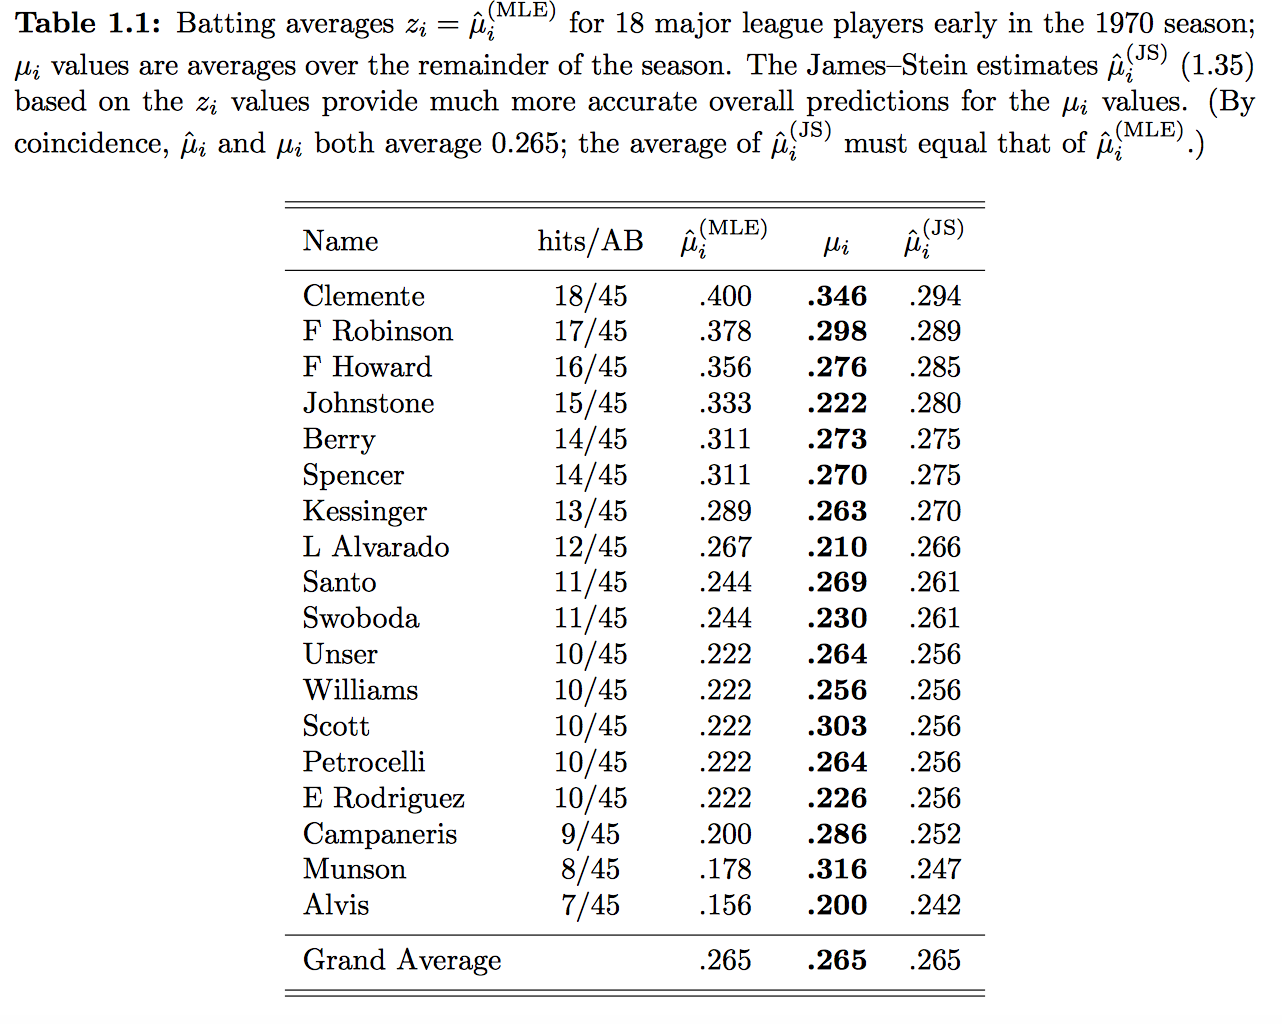
\includegraphics[width=3.5in]{./resources/baseball.png}
\end{center}
\end{frame}

\begin{frame}[fragile]{A (famous) Baseball Example}
Probably we can do better than the MLE here:
\begin{itemize}
\item Thurman Munson wins Rookie of the Year and ends up batting $\mu_i = .316$. If he batted .178 all year, his career would not have lasted long.
\item Clemente's $.400$ seems unlikely to hold up. Last player to hit $> .400$ was Ted Williams $.406$ in 1941.
\item But how?
\end{itemize}
\end{frame}

\begin{frame}[fragile]{Bayesian Shrinkage}
Idea is to take an average between the observed average $y_i$ and the overall mean $\overline{y}$:
\begin{align*}
\widehat{\mu}_i^{JS} &=  (1-\lambda) \cdot \overline{y}  + \lambda \cdot y_i, \quad
\lambda = 1 - \frac{(m-3) \sigma^2}{\sum_i( y_i - \overline{y})^2}
\end{align*}
\begin{itemize}
\item This has the effect of \alert{shrinking} $y_i$ towards the \alert{prior mean} $\overline{y}$.
\item In this case the \alert{prior mean} is just $\overline{y}$ the grand-mean of all players
\item How can information about unrelated players inform us about $\mu_i$?
\item Also consider proportion of foreign cars in Chicago as an additional $y_i$, can this help too?
\item The \alert{shrinkage factor} $\lambda$ depends on sample size and variance, but how is it chosen?
\end{itemize}
\end{frame}



\begin{frame}[fragile]{A Baseball Example}
\begin{center}
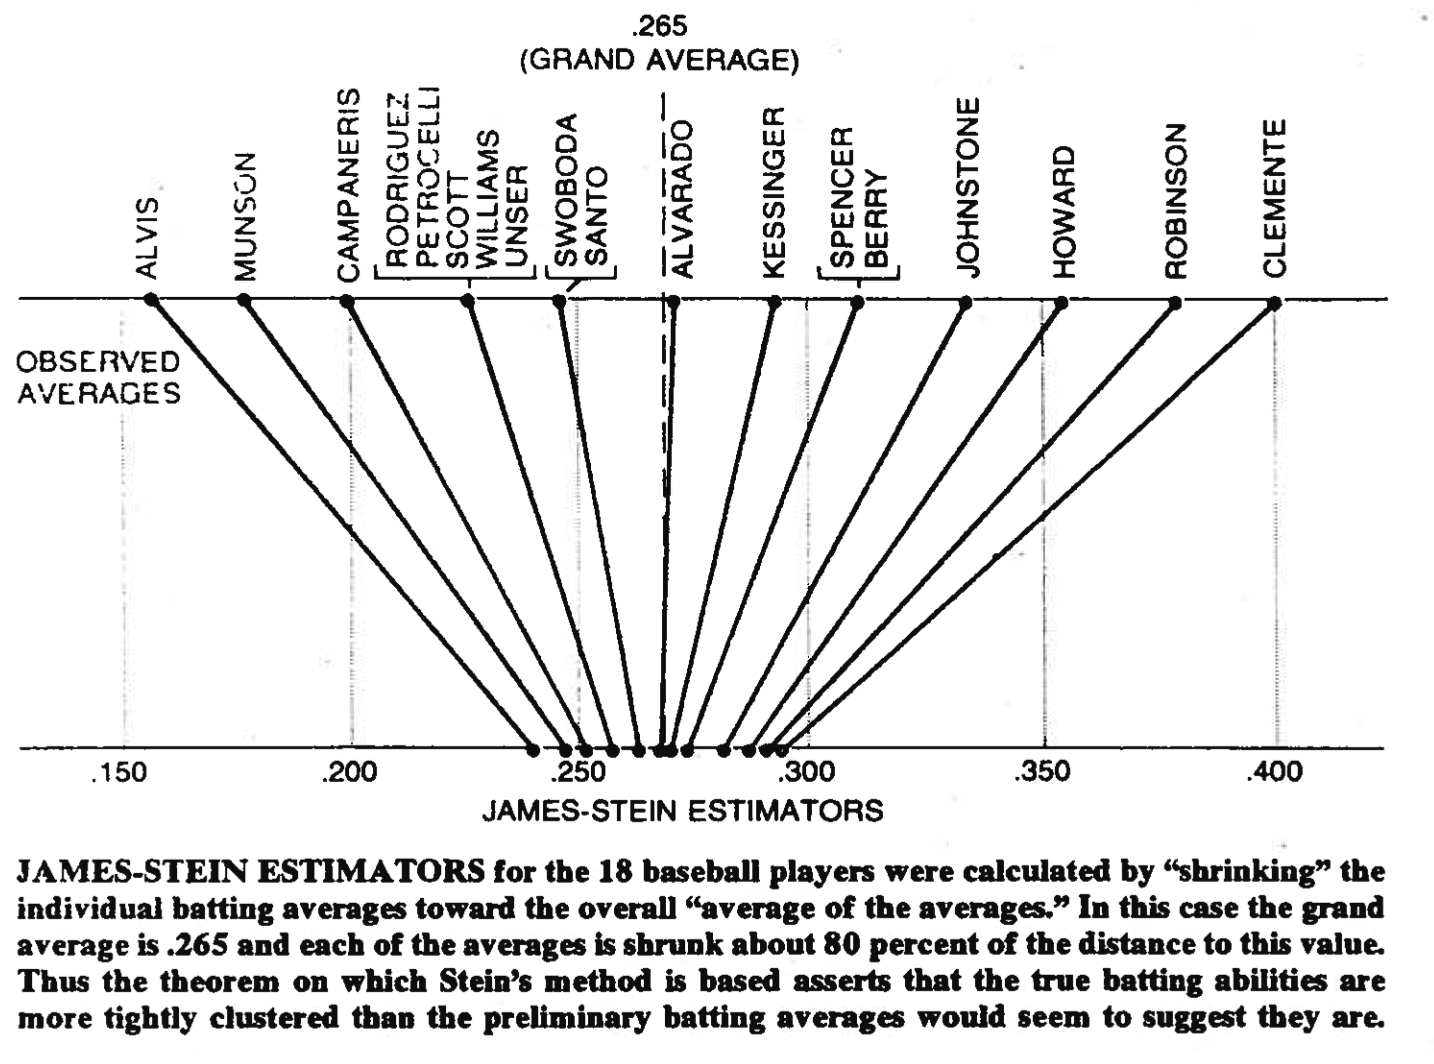
\includegraphics[width=3.5in]{./resources/baseball2.png}
\end{center}
\end{frame}

\section*{Thanks!}
\end{document}

\item We probably are interested in more observations $[x_1,\ldots,x_n]$ instead of just $x_1$.
\item $\sum_{i=1}^N x_i \sim Bin(N,p)$.